\documentclass[a4paper,12pt]{article}
\usepackage[margin=18mm]{geometry}
\usepackage{tikz}
\usepackage{amsmath}
\usepackage{xcolor}
\newcommand{\pFourCell}[2]{\makebox[#1em][c]{\ensuremath{#2}}}
\newcommand{\pFourCenterBox}[1]{\begingroup\setbox0=\hbox{$\displaystyle #1$}\dimen0=\ht0\advance\dimen0 by -\dp0\divide\dimen0 by 2\lower\dimen0\box0\endgroup}
\newdimen\pFourFractionRuleThickness
\pFourFractionRuleThickness=0.4pt
\newcommand{\pFourTopAlign}[3]{\raisebox{-#1}[0pt][\dimexpr #1 + #2\relax]{\ensuremath{\displaystyle #3}}}
\newcommand{\pFourBottomAlign}[3]{\raisebox{#2}[\dimexpr #1 + #2\relax][0pt]{\ensuremath{\displaystyle #3}}}
\newcommand{\pFourFractionInner}[2]{\hbox to #1{\hss$\displaystyle #2$\hss}}
\newcommand{\pFourFractionC}[4]{\begingroup\color{#1}\genfrac{}{}{\pFourFractionRuleThickness}{0}{\raisebox{0.14em}{\pFourFractionInner{#2}{{\color{black}#3}}}}{\raisebox{-0.18em}{\pFourFractionInner{#2}{{\color{black}#4}}}}\endgroup}
\newcommand{\pFourFraction}[3]{\genfrac{}{}{\pFourFractionRuleThickness}{0}{\raisebox{0.14em}{\pFourFractionInner{#1}{#2}}}{\raisebox{-0.18em}{\pFourFractionInner{#1}{#3}}}}
\newcommand{\pFourRootC}[2]{\begingroup\setbox0=\hbox{$\displaystyle #2$}\setbox2=\hbox{$\displaystyle \sqrt{\phantom{\copy0}}$}\dimen0=\wd2\advance\dimen0 by -\wd0\hbox{\rlap{\textcolor{#1}{\copy2}}\kern\dimen0\box0}\endgroup}
\newcommand{\pFourRoot}[1]{\pFourRootC{black}{#1}}
\newcommand{\pFourRootDegreeC}[3]{\begingroup\setbox0=\hbox{$\displaystyle #3$}\setbox2=\hbox{$\displaystyle \sqrt[#2]{\phantom{\copy0}}$}\dimen0=\wd2\advance\dimen0 by -\wd0\hbox{\rlap{\textcolor{#1}{\copy2}}\kern\dimen0\box0}\endgroup}
\newcommand{\pFourRootDegree}[2]{\pFourRootDegreeC{black}{#1}{#2}}
\pagestyle{empty}
\begin{document}

\section*{Spaltentreue LaTeX-Ausgabe}
\noindent Gleichung: \texttt{B}\texttt{\textasciicircum{}}\texttt{x}\texttt{=}\texttt{y}\texttt{/}\texttt{a} \hfill Zielvariable: \texttt{x} \hfill Profil: \texttt{standard}

\vspace{8mm}
\begin{center}
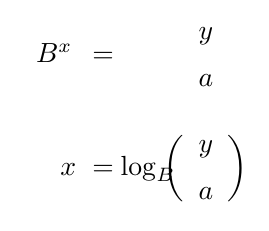
\begin{tikzpicture}[x=1em,y=-1em]
\node[anchor=base, inner sep=0pt] at (0.96,2.7) {$\pFourCell{1.92}{B^{{\scriptstyle x}}}$};
\node[anchor=base, inner sep=0pt] at (6.44,2.7) {$\pFourFraction{1.8em}{\makebox[1.8em][c]{\ensuremath{\pFourCell{0.9}{y}}}}{\makebox[1.8em][c]{\ensuremath{\pFourCell{0.9}{a}}}}$};
\node[anchor=base, inner sep=0pt] at (2.73,2.7) {$\pFourCell{1.62}{=}$};
\node[anchor=base, inner sep=0pt] at (6.44,6.78) {$\pFourFraction{1.8em}{\makebox[1.8em][c]{\ensuremath{\pFourCell{0.9}{y}}}}{\makebox[1.8em][c]{\ensuremath{\pFourCell{0.9}{a}}}}$};
\node[anchor=base, inner sep=0pt] at (1.47,6.78) {$\pFourCell{0.9}{x}$};
\node[anchor=base, inner sep=0pt] at (2.73,6.78) {$\pFourCell{1.62}{=}$};
\node[anchor=base, inner sep=0pt] at (4.35,6.78) {$\pFourCell{1.62}{\pFourCell{1.62}{\log_{B}}}$};
\node[anchor=base, inner sep=0pt] at (5.35,6.78) {$\pFourCell{0.38}{\left(\rule[-1em]{0pt}{1.96em}\right.}$};
\node[anchor=base, inner sep=0pt] at (7.53,6.78) {$\pFourCell{0.38}{\left.\rule[-1em]{0pt}{1.96em}\right)}$};
\end{tikzpicture}
\end{center}


\newpage
\section*{Spaltentreue LaTeX-Ausgabe mit Spaltengrenzen}
\vspace{6mm}
\begin{center}
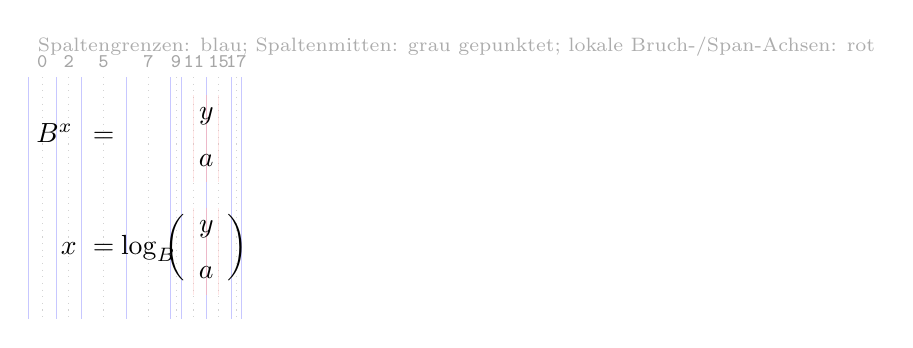
\begin{tikzpicture}[x=1em,y=-1em]
\node[font={\scriptsize}, text=gray!65, anchor=west] at (0,-0.75) {Spaltengrenzen: blau; Spaltenmitten: grau gepunktet; lokale Bruch-/Span-Achsen: rot};
\draw[blue!22, line width=0.28pt] (0,0.35) -- (0,9.11);
\draw[blue!22, line width=0.28pt] (1.02,0.35) -- (1.02,9.11);
\draw[blue!22, line width=0.28pt] (1.92,0.35) -- (1.92,9.11);
\draw[blue!22, line width=0.28pt] (3.54,0.35) -- (3.54,9.11);
\draw[blue!22, line width=0.28pt] (5.16,0.35) -- (5.16,9.11);
\draw[blue!22, line width=0.28pt] (5.54,0.35) -- (5.54,9.11);
\draw[blue!22, line width=0.28pt] (6.44,0.35) -- (6.44,9.11);
\draw[blue!22, line width=0.28pt] (7.34,0.35) -- (7.34,9.11);
\draw[blue!22, line width=0.28pt] (7.72,0.35) -- (7.72,9.11);
\draw[gray!35, dotted] (0.51,0.35) -- (0.51,9.11);
\node[font={\ttfamily\scriptsize}, text=gray!70, anchor=base] at (0.51,0) {0};
\draw[gray!35, dotted] (1.47,0.35) -- (1.47,9.11);
\node[font={\ttfamily\scriptsize}, text=gray!70, anchor=base] at (1.47,0) {2};
\draw[gray!35, dotted] (2.73,0.35) -- (2.73,9.11);
\node[font={\ttfamily\scriptsize}, text=gray!70, anchor=base] at (2.73,0) {5};
\draw[gray!35, dotted] (4.35,0.35) -- (4.35,9.11);
\node[font={\ttfamily\scriptsize}, text=gray!70, anchor=base] at (4.35,0) {7};
\draw[gray!35, dotted] (5.35,0.35) -- (5.35,9.11);
\node[font={\ttfamily\scriptsize}, text=gray!70, anchor=base] at (5.35,0) {9};
\draw[gray!35, dotted] (5.99,0.35) -- (5.99,9.11);
\node[font={\ttfamily\scriptsize}, text=gray!70, anchor=base] at (5.99,0) {11};
\draw[gray!35, dotted] (6.89,0.35) -- (6.89,9.11);
\node[font={\ttfamily\scriptsize}, text=gray!70, anchor=base] at (6.89,0) {15};
\draw[gray!35, dotted] (7.53,0.35) -- (7.53,9.11);
\node[font={\ttfamily\scriptsize}, text=gray!70, anchor=base] at (7.53,0) {17};
\node[anchor=base, inner sep=0pt] at (0.96,2.7) {$\pFourCell{1.92}{B^{{\scriptstyle x}}}$};
\draw[red!30, opacity=0.32, line width=0.35pt] (5.99,1) -- (5.99,4.13);
\draw[red!30, opacity=0.32, line width=0.35pt] (6.44,1) -- (6.44,4.13);
\draw[red!30, opacity=0.32, line width=0.35pt] (6.44,1) -- (6.44,4.13);
\draw[red!30, opacity=0.32, line width=0.35pt] (6.44,1) -- (6.44,4.13);
\draw[red!30, opacity=0.32, line width=0.35pt] (6.89,1) -- (6.89,4.13);
\node[anchor=base, inner sep=0pt] at (6.44,2.7) {$\pFourFraction{1.8em}{\makebox[1.8em][c]{\ensuremath{\pFourCell{0.9}{y}}}}{\makebox[1.8em][c]{\ensuremath{\pFourCell{0.9}{a}}}}$};
\node[anchor=base, inner sep=0pt] at (2.73,2.7) {$\pFourCell{1.62}{=}$};
\draw[red!30, opacity=0.32, line width=0.35pt] (5.99,5.08) -- (5.99,8.21);
\draw[red!30, opacity=0.32, line width=0.35pt] (6.44,5.08) -- (6.44,8.21);
\draw[red!30, opacity=0.32, line width=0.35pt] (6.44,5.08) -- (6.44,8.21);
\draw[red!30, opacity=0.32, line width=0.35pt] (6.44,5.08) -- (6.44,8.21);
\draw[red!30, opacity=0.32, line width=0.35pt] (6.89,5.08) -- (6.89,8.21);
\node[anchor=base, inner sep=0pt] at (6.44,6.78) {$\pFourFraction{1.8em}{\makebox[1.8em][c]{\ensuremath{\pFourCell{0.9}{y}}}}{\makebox[1.8em][c]{\ensuremath{\pFourCell{0.9}{a}}}}$};
\node[anchor=base, inner sep=0pt] at (1.47,6.78) {$\pFourCell{0.9}{x}$};
\node[anchor=base, inner sep=0pt] at (2.73,6.78) {$\pFourCell{1.62}{=}$};
\node[anchor=base, inner sep=0pt] at (4.35,6.78) {$\pFourCell{1.62}{\pFourCell{1.62}{\log_{B}}}$};
\node[anchor=base, inner sep=0pt] at (5.35,6.78) {$\pFourCell{0.38}{\left(\rule[-1em]{0pt}{1.96em}\right.}$};
\node[anchor=base, inner sep=0pt] at (7.53,6.78) {$\pFourCell{0.38}{\left.\rule[-1em]{0pt}{1.96em}\right)}$};
\end{tikzpicture}
\end{center}
\end{document}
